\chapter{Foundations}
	\label{c:foundations}
	\IMRADlabel{methods}

	\section{Dynamical Systems}
		A \emph{dynamical system}~\cite{birkhoffDynamicalSystems1927} is a (physical) system that evolves over time \(t\) and is completely defined by the values of \(n\) real variables
		\begin{align*}
			x_1, x_2, \,\cdots\!, x_n \quad\longleftrightarrow\quad \vec{x} = \begin{bmatrix} x_1 & x_2 & \cdots & x_m \end{bmatrix}^T
		\end{align*}
		called the \emph{state} and often written in vector form (right). Given the differentiability of these values, we can also study their rate of change (often referred to as the "velocity") and the rate of change of the rate of change (often referred to as the "acceleration"):
		\begin{align*}
			\dot{\vec{x}} = \dv{\vec{x}}{t} \qquad \ddot{\vec{x}} = \dv[2]{\vec{x}}{t}
		\end{align*}
		Describing these systems is possible using differential equations, both ordinary and partial ones. A general \ac{ode} is given by an implicit equation
		\begin{align}
			\vec{0} = \vec{F}\big( \vec{x}, \vec{x}^{(1)}, \vec{x}^{(2)}, \,\cdots\!, \vec{x}^{(k - 1)}, \vec{x}^{(k)}; t \big),\quad \vec{x}^{(l)} \coloneqq \dv[l]{\vec{x}}{t}  \label{eq:ode}
		\end{align}
		which establishes a connection between the state itself and its time derivatives. We call a function \( \vec{x}(t) \) a \emph{solution} of an \ac{ode} if its derivatives fulfill the given \ac{ode}~\eqref{eq:ode}. We will now employ some definitions and terms that we will use throughout the whole thesis.
		\begin{description}[leftmargin = 3cm]
			\item[Order] If \( \vec{x}^{(k)} \) is the derivative of highest order that appears in the \ac{ode}, the \ac{ode} is called to be of order \(k\).
			\item[Linearity] An \ac{ode} is \emph{linear} if \(\vec{F}\) is a linear function in terms of the state and its derivatives, \ac{ie} it is given as a linear combination
		\end{description}
		\begin{align*}
			\vec{F} = \vec{r}(t) + \sum_{i = 1}^{k} c_i(t) \vec{x}^{(i)},\quad \vec{r}(t) : \R \to \R^n,\, c_i(t) : \R \to \R
		\end{align*}
		\begin{description}[leftmargin = 3cm]
			\item[Autonomous] If \(\vec{F}\) explicitly is independent of \(t\) (\ac{ie} \( \pdv{\vec{F}}{t} = \vec{0} \)), the \ac{ode} is called \emph{autonomous}.
			\item[Homogenity] If no term  of \(\vec{F}\) is independent of the state or its derivatives, the \ac{ode} is called \emph{homogeneous}. For any homogeneous \ac{ode} one of its solutions is the trivial solution \( \vec{x} \equiv \vec{0} \).
		\end{description}

		In all of the following, we assume to have explicit, autonomous, first order \acp{ode}. This is valid because we can transform every explicit higher order \ac{ode} into a system of first order \acp{ode} as well as we can introduce another "time state" which makes our \ac{ode} autonomous.

		The solution theory for linear \acp{ode} is highly evolved and solutions exist for nearly every possible \ac{ode}. But for nonlinear \acp{ode}, the world looks different. With the exception of some rare cases, nonlinear \acp{ode} are not tractable. Hence, we often need approximations for the nonlinear case. Some well-known approaches for these approximations are \ac{eg} \emph{small angle approximation} for Sines and Cosines. In small angle approximations, we Taylor-expand \( \sin \)/\( \cos \) at \( \varphi_a = 0 \) and cut all higher order terms:
		\begin{gather*}
			\sin(\varphi) = \varphi - \underbrace{\frac{\varphi^3}{3!} + \frac{\varphi^5}{5!} + \cdots}_\text{higher order terms} \approx \varphi \\
			\cos(\varphi) = 1 - \underbrace{\frac{\varphi^2}{2!} + \frac{\varphi^4}{4!} - \frac{\varphi^6}{6!} + \cdots}_\text{higher order terms} \approx 1
		\end{gather*}
		This approach is illustrated in~\autoref{fig:smallAngleApproximation}.

		\begin{figure}
			\centering
			\begin{subfigure}[t]{0.5\linewidth}
				\centering
				\includegraphics[width = \linewidth]{figures/introduction/generated/small-angle-approximation-sin.pdf}
				\caption{Small angle approximation \( \sin(\varphi) \approx \varphi \) of Sine.}
			\end{subfigure}%
			~
			\begin{subfigure}[t]{0.5\linewidth}
				\centering
				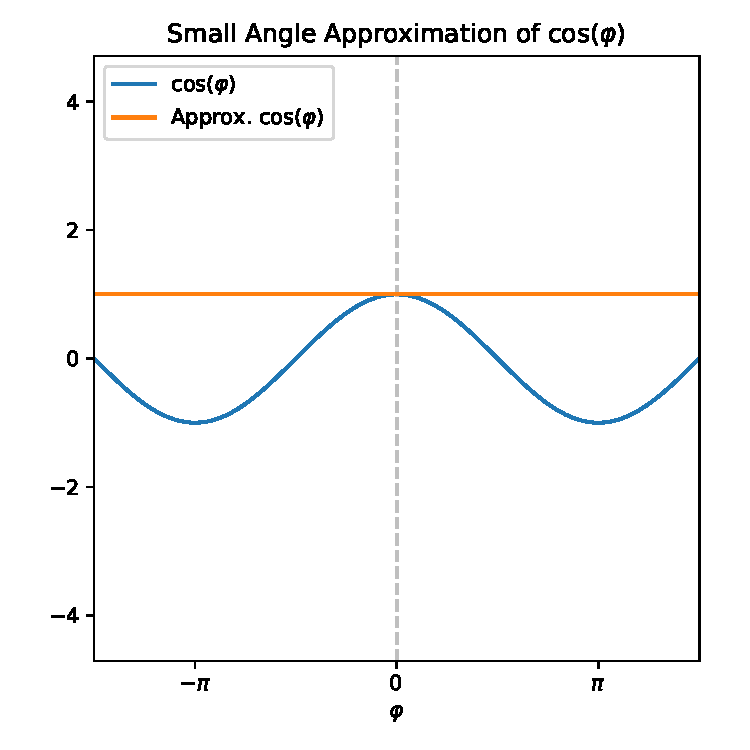
\includegraphics[width = \linewidth]{figures/introduction/generated/small-angle-approximation-cos.pdf}
				\caption{Small angle approximation \( \cos(\varphi) \approx 1 \) of Cosine.}
			\end{subfigure}
			\caption{Visualization of the small angle approximation (given is orange) of the basic trigonometric functions Sine and Cosine (given in blue). It is clear that the approximation is only valid in a small region around zero (\( \varphi \approx 0 \)).}
			\label{fig:smallAngleApproximation}
		\end{figure}

		We now look at two examples of dynamical systems, one which is linear and one that is not.

		\paragraph{Harmonic Oscillator}
			\label{subsec:harmonicOscillator}

			\begin{figure}
				\centering
				\tikzHarmonicOscillator
				\caption{Illustration of a simple harmonic oscillator with mass \(m\), spring stiffness \(k\) and position \(x\) that is not affected by any external force like gravity. The mass is in equilibrium if \( x = 0 \).}
				\label{fig:simpleHarmonicOscillator}
			\end{figure}

			The \emph{simple harmonic oscillator} describes the dynamical system of a mass \(m\) that is attached to a spring that is following Hooke's Law with stiffness \(k\) (see~\autoref{fig:simpleHarmonicOscillator}). This harmonic oscillator is described by the \ac{ode}
			\begin{align}
				m\ddot{x} = -kx \quad\iff\quad \ddot{x} = -\frac{k}{m} x  \label{eq:harmonicOscillator}
			\end{align}
			where \(x\) and \(\ddot{x}\) are the position and acceleration of the mass, respectively. Note that if \( x = 0 \), the mass is in equilibrium and no force is acting on it.

			By using basic results in the solution theory of linear \acp{ode}, we see that the general solution is given as
			\begin{align*}
				x(t) = A \cos\Big(t \sqrt{k / m} + \varphi\Big)
			\end{align*}
			with the amplitude \(A\) and the phase \(\varphi\) (see~\autoref{app:harmonicOscillatorSolution} for the derivation of the solution). As neither gravity nor damping or other external forces are involved in the dynamical system, the motion continues forever with a non-changing amplitude.
		% end

		\paragraph{Simple Pendulum}
			\label{subsec:simplePendulum}

			\begin{figure}
				\centering
				\tikzSimplePendulum
				\caption{Illustration of an inverse pendulum with mass \(m\) and displacement \(\varphi\) that is only affected by gravity and no other external force. The mass is in equilibrium for both \( \varphi = 0 \) and \( \varphi = \pi \), where the former is an unstable equilibrium.}
				\label{fig:simplePendulum}
			\end{figure}

			The \emph{inverse pendulum} described the dynamical system of a mass \(m\) that is attached to a rigid pole of length \(L\) which can freely swing around a suspension point (see~\autoref{fig:simplePendulum}). The pendulum stands upright if \( \varphi = 0 \) and its equation of motion is described by the \ac{ode}
			\begin{align*}
				\ddot{\varphi} = \frac{g}{L} \sin(\varphi)
			\end{align*}
			where \(g\), \(L\), \(\varphi\) and \(\ddot{\varphi}\) describe the gravity acceleration, pole length, displacement and acceleration of the mass, respectively. Note that if \( \varphi = 0 \), the mass is in an unstable equilibrium and no force is acting on it.

			In comparison to the harmonic oscillator (\autoref{subsec:harmonicOscillator}), this differential equation is nonlinear. And, even for the case with unit gravity acceleration \( g = 1 \) and unit pole length \( L = 1\), where the \ac{ode} looks really simple
			\begin{align}
				\ddot{\varphi} = \sin(\varphi)  \label{eq:inversePendulum}
			\end{align}
			it is not tractable analytically (\ac{ie} there exists no solution in closed form).

			Still, we can apply the small angle approximation introduced before (in this case, \( \sin(\varphi) \approx \varphi \)) which yields the simple equation
			\begin{align}
				\ddot{\varphi} \approx \varphi  \label{eq:linearizedInversePendulum}
			\end{align}
			which is solved by
			\begin{align*}
				\varphi(t) = \frac{1}{2} e^{-t} \big(\varphi_0 + e^{2t} \varphi_0 - \dot{\varphi}_0 + e^{2t} \dot{\varphi}_0\big)
			\end{align*}
			where \(\varphi_0\) and \(\dot{\varphi}_0\) are the initial displacement and velocity, respectively.

			However, this small angle approximation can only forecast small displacements \( \varphi \ll \pi/2 \). And, as the equilibrium at \( \varphi = 0 \) is unstable, the approximation becomes worst and worst as time goes on because the pendulum falls down. This behavior is shown in~\autoref{fig:inversePendulumApprox}.

			\begin{figure}
				\centering
				\begin{subfigure}[t]{0.5\linewidth}
					\centering
					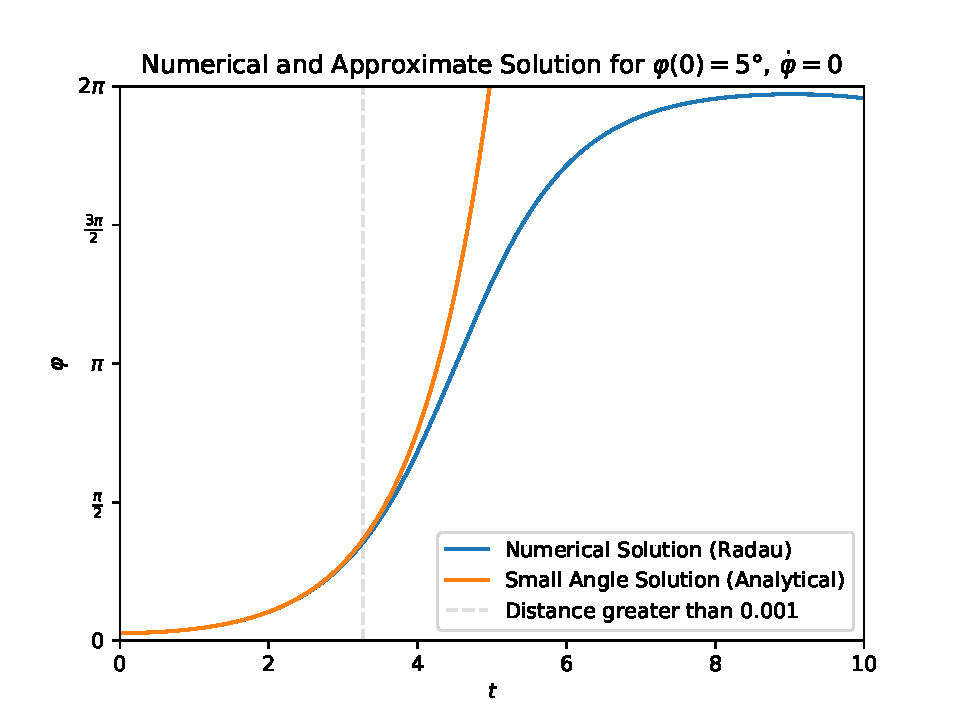
\includegraphics[width = \linewidth]{figures/introduction/generated/pendulum-motion-solutions}
					\caption{Trajectories of two solution strategies to the inverse pendulum, where the blue is a numerical solution of the actual motion of equation (solved using the Radau~IIA method~\cite[72]{hairerSolvingOrdinaryDifferential1996}) and the orange one is the analytically computed solution linearized \ac{ode}. The latter is linearized using small angle approximation. The dotted gray vertical line shows when the distance tolerance of \( \varepsilon = 10^{-3} \) is exceeded.}
				\end{subfigure}%
				~
				\begin{subfigure}[t]{0.5\linewidth}
					\centering
					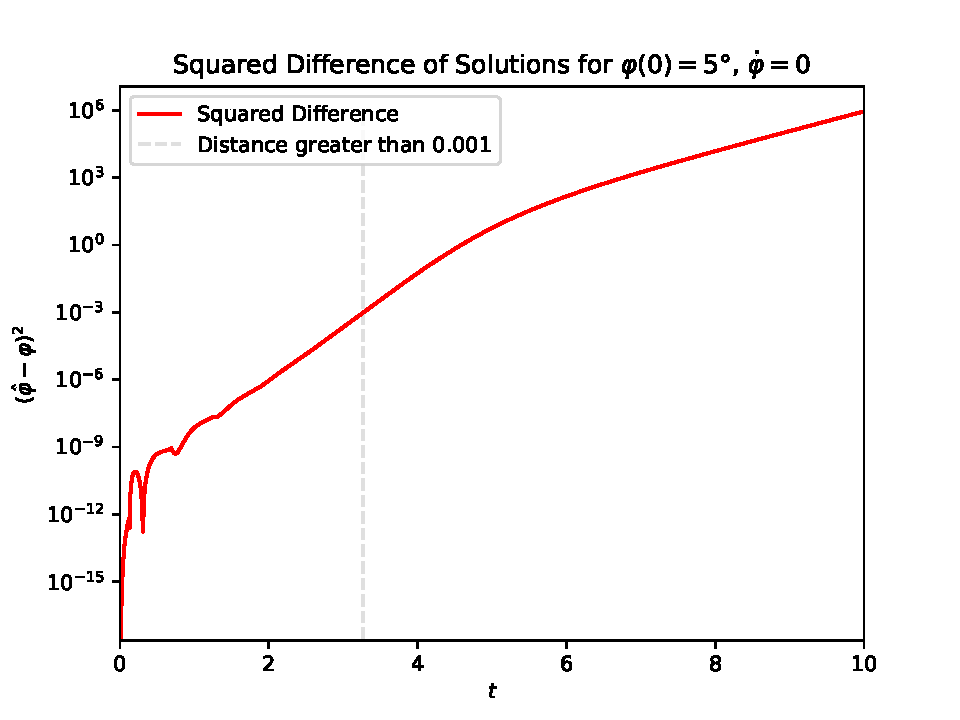
\includegraphics[width = \linewidth]{figures/introduction/generated/pendulum-motion-difference}
					\caption{Differences between the small angle approximation and the numerical solution of the \ac{ode}  The dotted gray vertical line shows when the distance tolerance of \( \varepsilon = 10^{-3} \) is exceeded.}
				\end{subfigure}
				\caption{Comparison of a numerical solution to the \ac{ode} of the inverse pendulum given in\eqref{eq:inversePendulum} and the analytical solution of the linearized \ac{ode} given in\eqref{eq:linearizedInversePendulum}. A tolerance value of \( \varepsilon = 10^{-3} \) is used to show when the both solutions diverge from each other.}
				\label{fig:inversePendulumApprox}
			\end{figure}
		% end

		\paragraph{Discrete-Time Dynamical Systems}
			In comparison to continuous-time dynamical systems described by \acp{ode}, discrete-time systems are described by a \emph{dynamics function} \( \vec{F} : \R^n \to \R^n \) advancing all states forward in time:
			\begin{align*}
				\vec{x}_{t + 1} = \vec{F}(\vec{x}_t)
			\end{align*}
			But we should note that, while seeming more restrictive, discrete-time dynamical systems are more general that continuous-time systems as we can discretize every continuous-time system
			\begin{align*}
				\dot{\vec{x}} = \vec{f}(\vec{x})
			\end{align*}
			as a discrete-time dynamical system
			\begin{align*}
				\vec{x}_{t + 1} = \vec{F}(\vec{x}_t)
			\end{align*}
			using the state dynamics function
			\begin{align*}
				\vec{F}\big(\vec{x}(t_0)\big) = \vec{x}(t_0 + \Delta_t) = \vec{x}(t_0) + \int_{t_0}^{t_0 + \Delta_t} \! \vec{f}\big(\vec{x}(\tau)\big) \dd{\tau}
			\end{align*}
			where \( \Delta_t \) is called the \emph{discretization interval} and \( \vec{x}_k = \vec{x}(k \Delta_t) \). Note that, from the Nyquist-Shannon sampling theorem, we now for band-limited functions that the sampling rate \( f_s = 1/\Delta_t \) has to be greater than two times the maximum frequency of the original function~\cite{shannonCommunicationPresenceNoise1949}, \ac{ie} \( f_s = 1/\Delta_t > 2 f \).
		% end

		\subsection{Koopman Dynamical Systems and the Koopman Operator}
			As we have seen, classical linearization approaches like the small angle approximation are only valid in a narrow section around the linearization point. While this works well for simple control tasks such as swinging up and balancing an inverted pendulum~\cite{bugejaNonlinearSwingupStabilizing2003}, it does not work out for predicting future trajectories of the system. % TODO: Citation needed.

			Consider a first-order, autonomous dynamical system
			\begin{align*}
				\dot{\vec{x}} = \vec{f}(\vec{x}),\quad \vec{f} : \R^n \to \R^n
			\end{align*}
			and observables ("measurements") \( \vec{g} : \R^n \to \R^m \). The Koopman operator \( \mathcal{K} \), an infinite-dimensional linear operator, acts on them as follows:
			\begin{align*}
				\mathcal{K} \vec{g} = \vec{g} \circ \vec{F} \quad\iff\quad \mathcal{K} \vec{g}(\vec{x}_t) = \vec{g}\big(\vec{F}(\vec{x}_t)\big) = \vec{g}(\vec{x}_{t + 1})
			\end{align*}
			In other words, the the Koopman operator advances our observables \(\vec{g}\) linearly forward in time. This behavior is illustrated in~\autoref{fig:koopmanOperatorBrunton}.

			The Koopman operator can also be formulated for time-continuous systems~\cite{abrahamManifoldsTensorAnalysis2012}:
			\begin{align*}
				\dv{t} \vec{g} = \mathcal{K} \vec{g}
			\end{align*}

			% TODO: Further explain Koopman theory after reading the corresponding sections in the Abraham book.

			\begin{figure}
				\centering
				\tikzKoopmanOperator
				\caption{Illustration of a Koopman dynamical system where time flows from left to right. The top row shows the linear embedding with the Koopman operator \( \mathcal{K} \) to transition from \(\vec{y}_t\) to \(\vec{y}_{t + 1}\). The bottom row shows the nonlinear dynamics produced by the dynamics function \(\vec{F}\). The measurement function \(\vec{g}\) allows transitioning between the two representations of the system state where \(\vec{g}^{-1}\) describes an "inverse" measurement function to recover the original nonlinear state from the linear embedding. We would like to find such a function. Adopted from~\cite{bruntonKoopmanInvariantSubspaces2016}.}
				\label{fig:koopmanOperatorBrunton}
			\end{figure}
		% end
	% end

	\section{Hidden Markov Models and Linear Gaussian Dynamical Systems}
		\subsection{Hidden Markov Models}
			\label{subsec:hiddenMarkovModel}

			\acp{hmm} are simple Bayesian networks described by a non-observable (\emph{hidden}) Markov chain. This non-observable discrete chain can be indirectly observed with measurements that are emitted by every state. One of the key features of a Markov chain is that a state does only depend on the previous state, but not on the second previous, third previous, and so on, states. That is, knowing only the previous state is sufficient and no more information can be gathered by knowing every other state before. This is described by the state transition distribution
			\begin{align*}
				s_{k + 1} \sim p(s_{k + 1} \given s_k)
			\end{align*}
			being only dependent on the previous state \(s_k\). Analogous, a measurement \(\vec{y}_k\) of a state \(s_k\) is only dependent on that specific state:
			\begin{align*}
				\vec{y}_k \sim p(\vec{y}_k \given s_k)
			\end{align*}
			These assumptions are called the \emph{Markov property} and a system fulfilling this property is called \emph{Markovian}. These conditional distributions can be written in a graphical model as shown in~\autoref{fig:hiddenMarkovModel}. Note that, in general, no assumption has to be made on the "type" of state/observation (\ac{ie} whether it is a scalar, a vector or something completely different). Also, no assumption is made on the specific transition distributions, \acp{hmm} can also be used to model deterministic transitions using a Dirac delta distribution.

			\begin{figure}
				\centering
				\tikzHiddenMarkovModel
				\caption{Illustration of a completely general Hidden Markov Model with states \(s_k\) and emissions/observations \(\vec{y}_k\).}
				\label{fig:hiddenMarkovModel}
			\end{figure}
		% end

		\subsection{Linear Gaussian Dynamical Systems}
			A general time-discrete linear system is described by a state transition
			\begin{align*}
				\vec{x}_{t + 1} = \mat{A} \vec{x}_t
			\end{align*}
			with a dynamics matrix \(\mat{A}\). Using purely additive Gaussian zero-mean noise \( \vec{\epsilon} \sim \normal(\vec{0}, \mat{Q}) \) with covariance matrix \( \mat{\Sigma} \), the state transition becomes probabilistic:
			\begin{align*}
				\vec{x}_{t + 1} = \mat{A} \vec{x}_t + \vec{\epsilon} \quad\iff\quad \vec{x}_{t + 1} \sim \normal(\mat{A} \vec{x}_t, \mat{Q})
			\end{align*}
			With analogous defined measurements,
			\begin{align*}
				\vec{y}_t \sim \normal(\mat{C} \vec{x}_t, \mat{R})
			\end{align*}
			the dynamical system becomes a \ac{lgds}, which is very similar to the \ac{hmm} described in~\autoref{subsec:hiddenMarkovModel}. It can also be represented using a graphical model as shown in~\autoref{fig:lgds}. In fact, a \ac{lgds} is kind of a \ac{hmm}, except the states are not discrete but continuous.

			\begin{figure}
				\centering
				\tikzLinearGaussianDynamicalSystem
				\caption{Illustration of a Linear Gaussian Dynamical System with states \(\vec{x}_t\) and observations \(\vec{y}_t\). Solid arrows represent probabilistic dependency, where the matrix \(\mat{A}\) is the dynamics matrix indicating that the mean transitions linearly, so do the observations with the observation matrix \(\mat{C}\).}
				\label{fig:lgds}
			\end{figure}
		% end

		\subsection{Inference}
			% TODO: Stopped here.
		% end
	% end

	\section{The Expectation-Maximization Algorithm}
		The \ac{em} algorithm can be used for tackling the following optimization problem: Assuming some model with latent (hidden) states \(\vec{x}\), observations \(\vec{y}\) and model parameters \(\vec{\theta}\), we want to maximize the likelihood \( p(\vec{y} \given \vec{\theta}) \) \ac{wrt} the latent states \(\vec{x}\) and the parameters \(\vec{\theta}\). However, the marginal distribution
		\begin{align*}
			p(\vec{y} \given \vec{\theta}) = \int\! p(\vec{x}, \vec{y} \given \vec{\theta}) \dd{\vec{x}}
		\end{align*}
		is generally intractable. As usual on maximum likelihood approaches, it is useful to not maximize the likelihood directly, but to maximize the log-likelihood
		\begin{align*}
			\mathcal{L}(\vec{\theta}) \coloneqq \log p(\vec{y} \given \vec{\theta}) = \log \int\! p(\vec{x}, \vec{y} \given \vec{\theta}) \dd{\vec{x}}
		\end{align*}
		instead. This yields the same maximum as the logarithm is strictly increasing. By introducing an auxiliary probability distribution \( q(\vec{x}) \) over the latent variables, we can rewrite the marginal and find a lower bound on \(\mathcal{L}\) by using Jensen's inequality~\cite{jensenFonctionsConvexesInegalites1906}:
		\begin{align*}
			\mathcal{L}(\vec{\theta})
				&= \log \int\! p(\vec{x}, \vec{y} \given \vec{\theta}) \dd{\vec{x}} \\
				&= \log \int\! q(\vec{x}) \frac{p(\vec{x}, \vec{y} \given \vec{\theta})}{q(\vec{x})} \dd{\vec{x}} \\
				&\geq \int\! q(\vec{x}) \log \frac{p(\vec{x}, \vec{y} \given \vec{\theta})}{q(\vec{x})} \dd{\vec{x}} \\
				&= \int\! q(\vec{x}) \log \frac{p(\vec{y} \given \vec{x}, \vec{\theta}) p(\vec{x} \given \vec{\theta})}{q(\vec{x})} \dd{\vec{x}} \\
				&= \int\! q(\vec{x}) \log p(\vec{y} \given \vec{x}, \vec{\theta}) + \int\! q(\vec{x}) \log \frac{p(\vec{x} \given \vec{\theta})}{q(\vec{x})} \dd{\vec{x}} \\
				&= \E_{q(\vec{x})}\big[ \log p(\vec{y} \given \vec{x}, \vec{\theta}) \big] - \KL{q(\vec{x})}{p(\vec{x} \given \vec{\theta})}
		\end{align*}
	% end

	\section{Variational Auto-Encoders and the Evidence Lower Bound}
	% end
% end
